\documentclass[12pt]{article}
\usepackage{graphicx} % Required for inserting images

% Refs and Bib
\usepackage{cite}               % order multiple entries in \cite{...}
\usepackage{breakurl}           % break too-long urls in refs
\usepackage{url}                % allow \url in bibtex for clickable links
\usepackage{xcolor}             % color definitions, to be use for...
\usepackage[]{hyperref}         % ...clickable refs within pdf...
\hypersetup{                    % ...like so
  colorlinks,
  linkcolor={green!80!black},
  citecolor={red!70!black},
  urlcolor={blue!70!black}
}

% \usepackage[%
%   backend=bibtex      % biber or bibtex
% %,style=authoryear    % Alphabeticalsch
%  ,style=numeric-comp  % numerical-compressed
%  ,sorting=none        % no sorting
%  ,sortcites=true      % some other example options ...
%  ,block=none
%  ,indexing=false
%  ,citereset=none
%  ,isbn=true
%  ,url=true
%  ,doi=true            % prints doi
%  ,natbib=true         % if you need natbib functions
% ]{biblatex}
% \addbibresource{refs.bib}  % better than \bibliography

% Paragraph indentation control
\usepackage{parskip}

% Papar margins
\usepackage[letterpaper,
            margin=1in,
            bottom=1in]{geometry}

% % Listing preferences
\usepackage{listings}
% \usepackage{color}

% \lstset{basicstyle=\footnotesize\ttfamily,breaklines=true}
% \lstset{framextopmargin=50pt,frame=bottomline}

\lstset
{ %Formatting for code in appendix
    basicstyle=\footnotesize\ttfamily,
    numbers=left,
    stepnumber=1,
    showstringspaces=false,
    % framextopmargin=50pt,
    tabsize=1,
    breaklines=true,
    breakatwhitespace=false,
    frame=bottomline
}

% %% Custom colors
% \definecolor{deepblue}{rgb}{0,0,0.5}
% \definecolor{deepred}{rgb}{0.6,0,0}
% \definecolor{deepgreen}{rgb}{0,0.5,0}

% % Python style for highlighting
% \newcommand\pythonstyle{\lstset{
% language=Python,
% basicstyle=\ttm,
% morekeywords={self},              % Add keywords here
% keywordstyle=\ttb\color{deepblue},
% emph={MyClass,__init__},          % Custom highlighting
% emphstyle=\ttb\color{deepred},    % Custom highlighting style
% stringstyle=\color{deepgreen},
% frame=tb,                         % Any extra options here
% showstringspaces=false
% }}
\usepackage{pythonhighlight}


% % Python environment
% \lstnewenvironment{python}[1][]
% {
% \pythonstyle
% \lstset{#1}
% }
% {}

% % Python for external files
% \newcommand\pythonexternal[2][]{{
% \pythonstyle
% \lstinputlisting[#1]{#2}}}

% % Python for inline
% \newcommand\pythoninline[1]{{\pythonstyle\lstinline!#1!}}

% Timeline
\usepackage{tikz}
\usetikzlibrary{fit, calc, decorations.markings}

% TODO: Change title to reflect changes in project.

% Title
% \title{Knowledge Graph Augmented Generative AI for Course Recommendation and Schedule Building}
% 
%% make title bold and 14 pt font (Latex default is non-bold, 16 pt)
\title{\Large \bf 
Knowledge Graph Querying for Course Schedule Building
}
% \title{\Large \bf 
% Knowledge Graph Augmented Generative AI for Course Recommendation and Schedule Building
% }

% Author(s) information
% \author{Adebayo Braimah}
\author{
{\rm Adebayo Braimah}\\
Stony Brook University \\
{\rm ID Number: 115099306}
% \and
% {\rm Author 2}\\
% Stony Brook University
}

% Date
% \date{March 2024}
\date{April 21, 2024}
% \date{\today}

% Variables
\def \repoLink{https://github.com/AdebayoBraimah/CSE505}
\def \docLink{https://cse505.readthedocs.io/en/latest/?badge=latest}
\def \desDocLink{https://docs.google.com/document/d/1t48in8rdzC_VOijfAOP23C_YgAQxkow5eaE7AXEVUYM/edit?usp=sharing}

% New commands
\newcommand*{\fullref}[1]{\hyperref[{#1}]{\autoref*{#1} \nameref*{#1}}}

\begin{document}
    
    % Title
    \maketitle
        
    \section{Problem \& Plan}
    \label{sec:prob_plan}
    
    \subsection{Problem Description}
    \label{subsec:problem}
    University course planning and understanding of graduation requirements can be a difficult process for new, in-coming students at all levels of one's education. Generally, new students are guided through this process by way of an academic advisor. However, this approach is expensive in both time and personnel (which are usually university faculty) -- especially in the case in which the personnel have to be trained on where to find and understand these graduation requirements. Additionally, in some cases -- the advising can be further complicated by the student's own personal interests (e.g. research focus, specific areas of interests, etc). The proposed solution to this problem would be knowledge graphs that are queried for course schedule building. A summary of the inputs and outputs are shown below:

    \subsubsection{Input \& Output}
    \label{subsubsec:in-out}
    
    \textbf{Inputs}:

    \begin{itemize}
        \label{items:inputs}
        \item Major
        \item Degree level(s): bachelors, masters, doctorate
        \item Current degree progress (e.g. classes already taken)
        \item Preferred classes
        \item Preferred graduation timeline
        \item Knowledge graphs
        \begin{itemize}
            \item Graduation requirements
            \item Department policies (e.g. restrictions on pass/fail courses)
            % Policy links:
            % https://www.cs.stonybrook.edu/sites/default/files/drupalfiles/basicpage/Undergraduate%20Policies.pdf
            % https://www.cs.stonybrook.edu/sites/default/files/drupalfiles/basicpage/Professional%20Ethics.pdf
        \end{itemize}
    \end{itemize}

    \textbf{Outputs}:

    \begin{itemize}
        \label{items:outputs}
        \item Recommended schedules
        \item Course recommendations
    \end{itemize}

    % Requirements
    \subsubsection{Requirements}
    \label{subsubsec:reqs}
    The requirements for this project would include:

    \begin{itemize}
        \item Tools
        \begin{itemize}
            \item Python
            \begin{itemize}
                \item Selenium (for web scraping)
                \item Pandas\cite{pandas} (for organizing data)
                \item webdriver-manager (web browser interface)
            \end{itemize}
            \item Clingo (ASP\footnote{Answer Set Programming} solver)\cite{clingo}
            % \item ErgoAI (Knowledge graph (KG) querying)
            % \item LLMs (large language models, multiple are shown -- likely only one will be used)
            % \begin{itemize}
            %     \item LLaMA\cite{touvron2023llama}/LLaMA-2\cite{touvron2023llama2}
            %     \item Alpaca\cite{alpaca}
            %     \item Chat-GPT 3.5-turbo\cite{ye2023gpt3.5}
            % \end{itemize}
        \end{itemize}
        \item Performance evaluation
            \begin{itemize}
                \item Measure the time and accuracy of each query and compare it to Stony Brook University's schedule builder\cite{sched}
            \end{itemize}
        \item Comparison of solutions
            \begin{itemize}
                \item Compare the output of the course schedules and recommendations with Stony Brook University graduation requirements (for computer science majors).
            \end{itemize}
    \end{itemize}
    
    % example uses
    \subsubsection{Example use-cases}
    \label{subsubsec:example}
    Moreover, the use cases of these solutions from this project are widely applicable to Stony Brook University's undergraduate, and graduate student populations as a whole. For example, these groups of students would find significant utility from this project's solutions:
    \begin{itemize}
        \item An undergraduate computer science student looking to meet the graduation requirements for a combined BS/MS in 5 years.
        \item A MS graduate student in the computer science department looking to satisfy graduation requirements in 2 years, taking 9--12 credits per semester.
        \item A computer science PhD student looking to satisfy course and department policy requirements prior to candidacy.
    \end{itemize}

    Granted the above use-cases were for computer science students -- ideally, most of the Stony Brook University student population would derive some benefit from this project.

    \subsection{State of the art}
    \label{subsec:sota}
    Current state-of-the-art (SOTA) approaches for this problem at Stony Brook University includes the \href{https://you.stonybrook.edu/uaamedia/schedulebuilder/}{schedule builder}. In the case of the schedule builder -- it will mostly help students build a schedule, semester by semester\cite{sched}, but it will not recommend classes.

    \subsection{Tasks \& Sub-tasks}
    \label{subsec:tasks}
    Currently, this project has no relation to any external projects (both through adjacent course work and for research purposes). Below are the corresponding tasks and sub-tasks for the project:

    \begin{itemize}
        \item \textbf{Task 1}: Knowledge graph construction (via web scraping)
        \begin{itemize}
            \item \textbf{Sub-task 1.1}: Create knowledge graphs of Stony Brook University undergraduate and graduate computer science graduation requirements (including department policies)
        \end{itemize}
        \item \textbf{Task 2}: Build API
        \begin{itemize}
            \item \textbf{Sub-task 2.1}: Create output knowledge base that can be queried.
        \end{itemize}
        \item \textbf{Task 3}: Test \& Evaluate
        \begin{itemize}
            \item \textbf{Sub-task 3.1}: Perform and automate test queries using commonly asked questions
            \item \textbf{Sub-task 3.2}: Evaluate performance (query time and accuracy)
        \end{itemize}
    \end{itemize}

    % Put arrow figure on next page
    \newpage
    
    \subsection{Project plan} 
    \label{subsec:plan}
    
    The repository for the planned code base is located at this public \href{\repoLink}{GitHub repository}. Additionally, the planned timeline of the project is shown below in \fullref{tikz:timeline}, with each set of tasks and sub-tasks (subsection \ref{subsec:tasks}) as checkpoints.
    
    % See this StackOverflow answer for further details:
% https://stackoverflow.com/a/77796855

%Curved Timeline
\begin{tikzpicture}[remember picture, overlay, shift={(8,-3)}]

  %Define control points for the first S-shaped curve
  \coordinate (start) at (-4, 0);
  \coordinate (control1) at (6, -3);
  \coordinate (middle) at (0, -7);
  \coordinate (end1) at (-6, -11);

  % Draw the first S-shaped curve
  \draw(start) .. controls (control1) .. (middle) .. controls (middle) and (end1) .. (end1);

  % Optional: Add labels to the control points for the first curve
  %\filldraw [purple] (start) circle (2pt) node[below] {Start};
  %\filldraw [red] (control1) circle (2pt) node[left] {Control 1};
  %\filldraw [red] (middle) circle (2pt) node[above] {Middle};
  %\filldraw [red] (end1) circle (2pt) node[below] {End 1};

  % Define control points for the second S-shaped curve
  \coordinate (control3) at (8, -2.5);
  \coordinate (middle2) at (4, -6.5);
  \coordinate (end2) at (-3, -14);

  % Draw the second S-shaped curve with an arrow at the end
  \draw (start) .. controls (control3) .. (middle2) .. controls (middle2) and (end2) .. (end2);

  % Optional: Add labels to the control points for the second curve
  %\filldraw [blue] (control3) circle (2pt) node[right] {Control 3};
  %\filldraw [blue] (middle2) circle (2pt) node[below] {Middle 2};
  %\filldraw [blue] (end2) circle (2pt) node[above] {End 2};

  %General coordinates
  \coordinate (arrow1) at ($(end1) + (-1, +1)$);
  \coordinate (arrow2) at ($(end2) + (+1, -1)$);
  \coordinate (arrow3) at ($(arrow2) + (-5.3, 0)$);

  % Optional: Add labels to the control points for the arrow head
  %\filldraw [green] (arrow1) circle (2pt) node[below] {Arrow 1};
  %\filldraw [green] (arrow2) circle (2pt) node[above] {Arrow 2};
  %\filldraw [green] (arrow3) circle (2pt) node[above] {Arrow 3};

  %Draw the arrow head
  \draw (end1) -- (arrow1) -- (arrow3) -- (arrow2) -- (end2);

 %Shade the region between the two curves
 \begin{scope}
    \shade[bottom color=blue!10, top color=blue!60, opacity=0.8] 
      (arrow3) -- (arrow2) -- (end2) -- (middle2) .. controls (control3) .. (start) .. controls (control1) .. (middle) .. controls (middle) and (end1) .. (end1) -- (arrow1) -- (arrow3) -- cycle;
  \end{scope}

  % Define control points for the curved path
  \coordinate (pathControl) at ($(control1)!0.5!(control3)$);
  \coordinate (pathMiddle) at ($(middle)!0.5!(middle2)$);
  \coordinate (pathEnd) at (arrow3);
  \coordinate (pathEnd2) at ($(end1)!0.5!(end2)$);

  % Draw the curved path
  %\filldraw [yellow] (pathControl) circle (2pt) node[below] {Path Control};
  %\filldraw [yellow] (pathMiddle) circle (2pt) node[below] {Path Middle};
  %\filldraw [yellow] (pathEnd) circle (2pt) node[below] {Path End};
  %\filldraw [yellow] (pathEnd2) circle (2pt) node[below] {Path End2};
  %\draw[red] (start) .. controls (pathControl) .. (pathMiddle) .. controls (pathMiddle) and (pathEnd) .. (pathEnd2);
  %\draw[blue] (pathEnd2) -- (pathEnd);

  % Draw ovals at the starting point
  \draw[color = red, fill = red, opacity = 0.8, line width=0.01cm] ($(start) + (0.806, -0.2)$) ellipse [x radius=0.098cm, y radius=0.0225cm];
  \draw[color = orange, fill = orange, opacity = 0.8, line width=0.01cm] ($(start) + (4.2, -1.074)$) ellipse [x radius=0.436cm, y radius=0.155cm];
  \draw[color = cyan, fill = cyan, opacity = 0.8, line width=0.01cm] ($(start) + (6.85, -1.84)$) ellipse [x radius=0.77cm, y radius=0.27cm];
  \draw[color = green, fill = green, opacity = 0.8, line width=0.01cm] ($(start) + (9.23, -3.55)$) ellipse [x radius=1.135cm, y radius=0.5cm];
  \draw[color = teal, fill = teal, opacity = 0.8, line width=0.01cm] ($(start) + (7.31, -5.8)$) ellipse [x radius=1.22cm, y radius=0.65cm];
  \draw[color = blue, fill = blue, opacity = 0.8, line width=0.01cm] ($(start) + (5.02, -7.7)$) ellipse [x radius=1.72cm, y radius=0.75cm];
  \draw[color = purple, fill = purple, opacity = 0.8, line width=0.01cm] ($(start) + (2.1, -10.111)$) ellipse [x radius=2.36cm, y radius=0.95cm];

  % Draw ovals around the existing ovals with the same ratios
  \draw[color=red, line width=0.005cm] ($(start) + (0.806, -0.2)$) ellipse [x radius=0.098cm*1.575, y radius=0.0225cm*1.575];
  \draw[color=orange, line width=0.005cm] ($(start) + (4.2, -1.074)$) ellipse [x radius=0.436cm*1.5, y radius=0.155cm*1.5];
  \draw[color = cyan, line width = 0.005cm] ($(start) + (6.85, -1.84)$) ellipse [x radius=0.77cm*1.3, y radius=0.27cm*1.3];
  \draw[color = green, line width = 0.005cm] ($(start) +(9.23, -3.55)$) ellipse [x radius=1.135cm*1.3, y radius=0.5cm*1.3];
  \draw[color = teal, line width = 0.005cm] ($(start) + (7.31, -5.8)$) ellipse [x radius=1.22cm*1.3, y radius=0.65cm*1.3];
  \draw[color = blue, line width = 0.005cm] ($(start) + (5.02, -7.7)$) ellipse [x radius=1.72cm*1.25, y radius=0.75cm*1.25];
  \draw[color = purple, line width = 0.005cm] ($(start) + (2.1, -10.111)$) ellipse [x radius=2.36cm*1.2, y radius=0.95cm*1.2];

  % Draw perpendicular lines going up 3cm
  \draw[color = red, dashed, opacity = 1] ($(start) + (0.806, -0.2)$) -- ++(90:3.5cm) node[right, scale = 0.9, color = red] {Mar. 15, 2024};
  \draw[color = orange, dashed, opacity = 1] ($(start) + (4.2, -1.074)$) -- ++(90:3.5cm) node[right, scale = 0.9, color = orange] {Mar. 22, 2024};
  \draw[color = cyan, dashed, opacity = 1] ($(start) + (6.85, -1.84)$) -- ++(90:3.5cm) node[right, scale = 0.9, color = cyan] {Mar. 29, 2024};
  \draw[color = green, dashed, opacity = 1] ($(start) + (9.23, -3.55)$) -- ++(-90:3.5cm)  node[right, scale = 0.9, color = green] {April 05, 2024};
  \draw[color = teal, dashed, opacity = 1] ($(start) + (7.31, -5.8)$) -- ++(-90:3.5cm) node[right, scale = 0.9, color = teal] {April 19, 2024};
  \draw[color = blue, dashed, opacity = 1] ($(start) + (5.02, -7.7)$) -- ++(-90:4.5cm) node[right, scale = 0.9, color = blue] {April 26, 2024};
  \draw[color = purple, dashed, opacity = 1] ($(start) + (2.1, -10.111)$) -- ++(-90:4.5cm) node[right, scale = 0.9, color = purple] {May 03, 2024};

  % Add text under the years
  \node[right, color = black, scale = 1] (1) at ($(start) + (0.87, -0.2)  + (90:2.8cm)$) {\textbf{Phase 1}:};
  \node[right, color = black, scale = 1] (2) at ($(start) + (0.87, -0.32)  + (90:2.4cm)$) {1.1 \& 2.1};
  \node[right, color = black, scale = 1] (3) at ($(start) + (4.27, -1.074)  + (90:2.8cm)$) {\textbf{API}: (begin)};
  \node[right, color = black, scale = 1] (4) at ($(start) + (4.27, -1.074) + (90:2.4cm)$) {1.2, 2.1 -- 2.3};
  \node[right, color = black, scale = 1] (5) at ($(start) + (6.95, -1.84) + (90:2.8cm)$) {\textbf{API}: (end)};
  \node[right, color = black, scale = 1] (6) at ($(start) + (6.95, -1.84)+ (90:2.4cm)$) {1.2, 2.1 -- 2.3};
  \node[right, color = black, scale = 1] (7) at ($(start) + (6.95, -1.84) + (90:2cm)$) {(cont.)};
  \node[right, color = black, scale = 1] (8) at ($(start) + (9.38, -3.55) + (-90:2.4cm)$) {\textbf{Prototype}:};
  \node[right, color = black, scale = 1] (9) at ($(start) + (9.38, -3.55) + (-90:2.8cm)$) {2.2, 2.3, 3.1};
  \node[right, color = black, scale = 1] (10) at ($(start) + (7.36, -5.8) + (-90:2cm)$) {\textbf{Phase 2}:};
  \node[right, color = black, scale = 1] (11) at ($(start) + (7.36, -5.8) + (-90:2.4cm)$) {Prototype};
  \node[right, color = black, scale = 1] (12) at ($(start) + (7.36, -5.8) + (-90:2.8cm)$) {2.2, 2.3, 3.1};
  \node[right, color = black, scale = 1] (13) at ($(start) + (5.09, -7.7) + (-90:3cm)$) {\textbf{Test/Eval}:};
  \node[right, color = black, scale = 1] (14) at ($(start) + (5.09, -7.7) + (-90:3.4cm)$) {3.1, 3.2};
  \node[right, color = black, scale = 1] (15) at ($(start) + (5.09, -7.7) + (-90:3.8cm)$) {1.2 (if time)};
  \node[right, color = black, scale = 1] (16) at ($(start) + (2.25, -10.111) + (-90:3.4cm)$) {\textbf{Due Date}};
  \node[right, color = black, scale = 1] (17) at ($(start) + (2.25, -10.111) + (-90:3.8cm)$) {Submit project};

  % Draw a box around the text nodes with the same opacity
  \node[draw, line width = 0.005cm, rounded corners, scale = 0.85, fit={(1) (2)}] {};
  \node[draw, line width = 0.005cm, rounded corners, scale = 0.85, fit={(3) (4)}] {};
  \node[draw, line width = 0.005cm, rounded corners, scale = 0.85, fit={(5) (6) (7)}] {};
  \node[draw, line width = 0.005cm, rounded corners, scale = 0.85, fit={(8) (9)}] {};
  \node[draw, line width = 0.005cm, rounded corners, scale = 0.85, fit={(10) (11) (12)}] {};
  \node[draw, line width = 0.005cm, rounded corners, scale = 0.85, fit={(13) (14) (15)}] {};
  \node[draw, line width = 0.005cm, rounded corners, scale = 0.85, fit={(16) (17)}] {};
\end{tikzpicture}

% \end{document} \label{tikz:timeline} \newpage

    % Design docs
    % See this link for further details:
    % https://github.com/aws/aws-sam-cli/blob/develop/designs/intrinsics_design.md
    \section{Design}
    \label{sec:design}

    \subsection{API}
    \label{subsec:api}

    The API implementation can be summarized as shown in the UML\footnote{Unified Modeling Language} diagram in Figure \ref{fig:uml-package} in addition to class structures for {\tt{KnowledgeBase}} and {\tt{KnowledgeGraph}} with their corresponding class attributes in Figure \ref{fig:uml-classes}.

    \begin{figure}[h!]
        \centering
        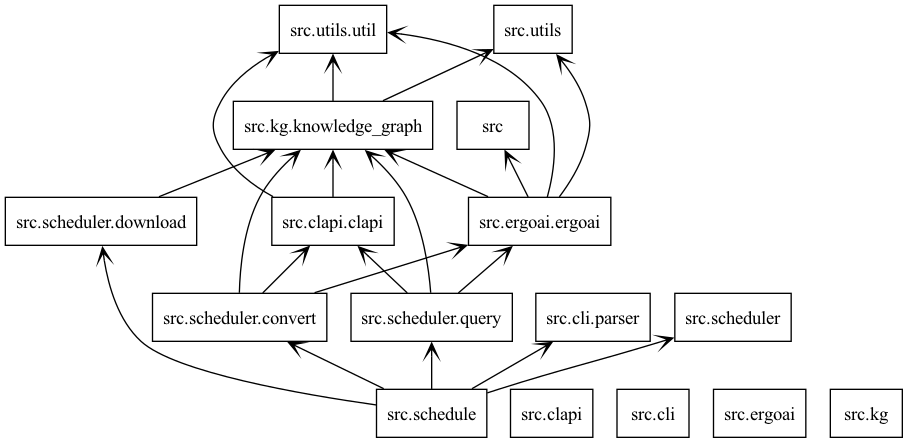
\includegraphics[scale=0.75]{figures/uml/packages_src.png}
        \caption{UML Diagram of the python package}
        \label{fig:uml-package}
    \end{figure}

    \begin{figure}[h!]
        \centering
        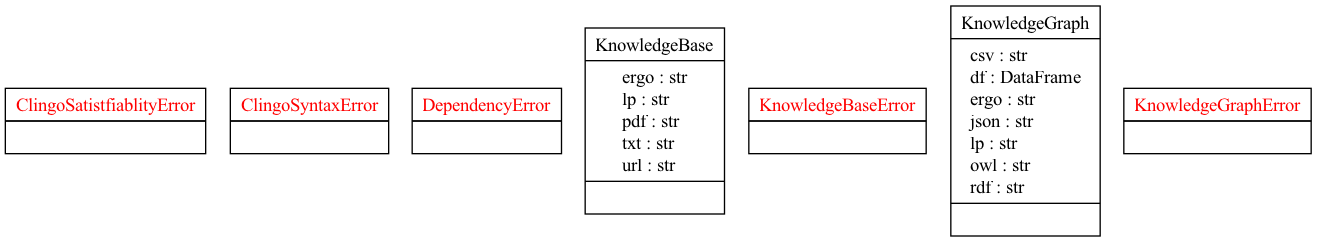
\includegraphics[scale=0.55]{figures/uml/classes_src.png}
        \caption{UML Diagram of the python package's classes and corresponding attributes.}
        \label{fig:uml-classes}
    \end{figure}

    The driver program of this project can be run as shown from the command line:

    {\tt{./app.py}}

    Note, that file permissions may need to be changed for the file to run.

    The outputs of the file are the results of the test query, printed to the command line (truncated version of the file {\tt{src/resources/cse.schedule.lp}}, thus the unsatisfiable result): \\

    \begin{verbatim}
        UNSATISFIABLE
        
        Models       : 0
        Calls        : 1
        Time         : 5.358s (Solving: 5.35s 1st Model: 0.00s Unsat: 5.35s)
        CPU Time     : 5.351s
    \end{verbatim}

    % \begin{python}
    % import os
    % from src.ergoai.ergoai import query_ergoai
    
    % test_file: str = os.path.abspath("foo.ergo")
    % query: str = "?Subject[?Property->?Object]"
    
    % query_ergoai(knowledge=test_file, query=query)
    % \end{python}

    \subsubsection{Implementation Details}
    \label{subsubsec:implementation}

    The implementation details of this project are depicted in the UML diagrams shown in Figures \ref{fig:uml-package} and \ref{fig:uml-classes}. Moreover, the module {\tt{src.schedule}} is the main entry point into this program and takes the following input:

    \begin{itemize}
        \item A {\tt{KnowledgeBase}} object or a  {\tt{KnowledgeGraph}} object.
        \begin{itemize}
            \item {\tt{KnowledgeBase}}: Containing URL.
            \item {\tt{KnowledgeGraph}}: Containing either a:
            \begin{itemize}
                \item JSON file
                \item ErgoAI file
                \item Clingo file
                \item URL
            \end{itemize}
        \end{itemize}
        \item Major (using Stony Brook's three designation, e.g. CSE)
        \item Method (i.e. solver/approach to be used): Clingo in this case.
    \end{itemize}
    

    \subsection{Third Party Libraries}
    \label{subsec:thirdparty}

    The third party libraries currently used (mentioned in \ref{subsubsec:in-out}) include Selenium (for web scraping), Pandas (data organization prior to writing knowledge graphs), webdriver-manager (for browser interface) and Clingo (ASP solver, installed via (mini)conda).

    \subsection{Documentation}
    \label{subsec:docs}

    The documentation of this project is contained in the {\tt{doc}} folder. Documentation was also written in reStructured Text ({\tt{.rst}}) files, and built using python via \href{https://www.sphinx-doc.org/en/master/}{Sphinx} ({\tt{HTML}} documentation can be found in {\tt{doc/build/html/index.html}}). The {\tt{HTML}} documentation can found online \href{\docLink}{here} (recommended method of viewing this documentation).

    \subsection{Design Document}
    \label{subsec:design-docs}

    The design document\footnote{Format referenced from this AWS design document in this \href{https://github.com/aws/aws-sam-cli/blob/develop/designs/intrinsics_design.md}{GitHub repository}} for this project is located \href{\desDocLink}{here in this Google Document}. The design document can be briefly summarized as:

    \begin{itemize}
        \item The project purpose: stating the problem, goals and those impacted (see section \ref{subsubsec:in-out}).
        \item Project scope: What features will be built, and what features will not be implemented.
        \item Stakeholders: The target audience, and those impacted by this project.
        \item Requirements: Functional and non-functional requirements (see section \ref{subsubsec:reqs}).
        \item Project timeline and milestones (see section \ref{subsec:plan}).
        \item Architecture and system design (see Figures \ref{fig:uml-package} \& \ref{fig:uml-classes})
        \item Test \& quality assurance: Test cases and queries that need to be covered.
    \end{itemize}
    
    \section{Implementation}
    \label{sec:implement}

    \subsection{Design Implementation}
    \label{subsec:des-imp}

    The current design implementation has focused on translating knowledge graphs into facts. Correspondingly, knowledge bases were translated into rules. For example, the the class information shown in the JSON snippet below,  could be translated into the following fact:

    \begin{lstlisting}
    {
        .
        .
        .
        "CSE 214":{
        "Course Title":"Data Structures",
        "Career":"Undergraduate",
        "Credits":4.0,
        "Prerequisites":[
            [
                "CSE 114"
            ]
        ]
    },
    "CSE 215":{
        "Course Title":"Foundations of Computer Science",
        "Career":"Undergraduate",
        "Credits":4.0,
        "Prerequisites":[
            [
                "AMS 151",
                "MAT 125",
                "MAT 131"
            ]
        ]
    },
    .
    .
    .
    }
    \end{lstlisting}

    Facts translation in Clingo (located in: {\tt{src/resources/cse.schedule.lp}})): \\
    
    \begin{lstlisting}
        % Clingo code
        % Define course(course_name, credits)
        course(cse214, 4).
        course(cse215, 4).
        .
        .
        .
        % Define prerequisites
        % prerequisite(course_name, prerequisite)
        prerequisite(cse214, cse114).
        prerequisite(cse215, ams151).
        prerequisite(cse215, mat125).
        prerequisite(cse215, mat131).
    \end{lstlisting}

    Correspondingly, the knowledge base facts were translated into rules. For example, the fact a student needs take a minimum of 12 credits a semester, but a maximum of 15 credits over a $N$ semesters to graduate with 80 credits would be translated as the following in Clingo (in the same file, {\tt{src/resources/cse.schedule.lp}}): \\

    \begin{lstlisting}
        % Constants
        min_credits_per_semester(12).
        max_credits_per_semester(15).
        total_required_credits(80).
        
        % Assign courses to semesters (1..N), N is an upper bound on semesters, guessed here as 10
        semester(1..10).
        
        % Assign a course to exactly one semester
        1 { in_semester(C, S) : semester(S) } 1 :- course(C, _).
        
        % Constraint to ensure the minimum number of credits per semester
        :- semester(S), min_credits_per_semester(Min), #sum{Credits, C : course(C, Credits), in_semester(C, S)} < Min.
        
        % Ensure the total credits in each semester do not exceed the maximum allowed
        :- semester(S), max_credits_per_semester(Max), #sum{Credits, C : course(C, Credits), in_semester(C, S)} > Max.
        
        % Ensuring all prerequisites are met
        :- course(C, _), in_semester(C, SC), prerequisite(C, P), course(P, _), in_semester(P, SP), SP >= SC.
        
        % Define the maximum semester used
        max_semester_used(M) :- M = #max{S : in_semester(_, S)}.
        
        % Minimize the number of semesters used
        #minimize{M : max_semester_used(M)}.
        
        % Output control
        #show in_semester/2.
    \end{lstlisting}


    \subsubsection{Design Issues \& Problems}
    \label{subsubsec:des-iss-probs}

    Currently, the way the queries are written are quite problematic. In addition to the rules and facts. As of right now, evaluation of the project is difficult. When the part of the knowledge graph consisting of undergraduate courses is used as input into Clingo (in the file {\tt{src/resources/cse.schedule.lp}}), the runtime was 37,801 secs. (10.5 hours)! The culprit is most likely in the way the queries have been written, in addition to the constraints. Conversely, ErgoAI would likely handle this problem much better -- however, translating facts into rules that can be queried with a knowledge graph has proven to be quite difficult.

    \subsection{Design Documents (updated)}
    \label{subsec:des-doc-up}

    See section \ref{subsec:design-docs} for a summary of the design document. The design document can also be found \href{\desDocLink}{here in this Google Document}. The design document at this link has been updated in accordance with the specifications of this project.

    \subsection{Project Implementation}
    \label{subsec:proj-imp}

    The project implementation can be found in the following code base, located at \href{\repoLink}{this GitHub Repository}. The development effort of the project required sizable effort -- especially in the parts pertaining to ErgoAI (which is not currently implemented). Below is a brief summary of the project:

    \begin{itemize}
        \item Languages
        \begin{itemize}
            \item Python
            \begin{itemize}
                \item Selenium
                \item Pandas
                \item webdriver-manager
            \end{itemize}
            \item Clingo
            \item ErgoAI (not implemented, but attempted)
        \end{itemize}
        \item Tools
            \begin{itemize}
                \item Conda (python environment management)
                \item Sphinx (automated documentation)
                \item Graphviz \& PyLint (for creating UML diagrams)
                \item Black (python code formatter)
            \end{itemize}
        \item Development effort: Fairly sizable, especially in reference to ErgoAI (not implemented).
        \item Code base size: moderately sized at 32,597 lines of code.
    \end{itemize}

    Lastly, this project, in its current state significantly lags behind the SOTA approaches.
    
    \section{Testing \& Evaluation}
    \label{sec:test_eval}

    No official tests have been run yet -- as evaluation has been difficult (see section \ref{subsubsec:des-iss-probs} for further details). In the project's current state, evaluation is a tricky endeavor. Moreover, the tests that remain to be written and performed include:

    \begin{itemize}
        \item Unit tests
        \item Reachability
        \item Cycle detection
        \item Performance \& Correctness
    \end{itemize}
    
    \section{Acknowledgements}
    \label{sec:ack}

    \begin{itemize}
        \item Prof. Annie Liu for the project idea and insights
        \item Geoffrey Churchill for discussions and insights
    \end{itemize}

    % TODO:
    %   - Update acknowledgements section
    %   - Include section that tracks changes or
    %       at least mentions what was changed 
    %       and why.

    % Add newpage here to separate references from the
    % main text body
    \newpage
    
    % Bibliography & References
    \bibliographystyle{acm}
    \bibliography{refs}
    
    % \printbibliography

    \newpage
    
    \section{Appendix}
    \label{sec:appendix}

    \subsection{Changelog (Change Log)}
    \label{subsec:change}

    % LLM
    % Project scope
    % Knowledge graph extraction
    % Course review/recommendation
    % Project external dependencies (link to documentation)
    % Python dependencies (link to relevant docs/websites)
    % Mention web-scraper

    \begin{itemize}
        \item Removed/exchanged these tools and features:
        \begin{itemize}
            \item Large Language Models (LLMs) were removed.
            \item Sub-graph extraction (via Neural State Machine for Knowledge Base Question Answering) was exchanged for just scraping Stony Brook's SOLAR course catalog for knowledge graph creation.
            \item Automated rule creation from knowledge base was removed (outside the scope of this project).
            \item Course reviews feature was removed.
            \item ErgoAI was exchanged for Clingo.
        \end{itemize}
        \item Design Document
        \begin{itemize}
            \item Linked a Google Document with the relevant information and details.
            \item Added UML diagrams to pictorially describe the project's code base.
            \item Added more explicit design and implementation details.
            \item Updated third party libraries and external dependencies used.
        \end{itemize}
    \end{itemize}

\end{document}
